\documentclass[a4paper,12pt,english]{all-in-one} %% TWOSIDE
\usepackage{ebgaramond}
\usepackage{amsmath} 
\usepackage{newtxmath}
\usepackage{multicol}
\usepackage{lipsum}
\usepackage{subfig}
\usepackage{listings}
\usepackage[hidelinks]{hyperref}

\doctitle{ Modern Physics Laboratory }
\docsubtitle{Zeeman Effect}

\makeatletter
\title{{\large\textit{Modern Physics Laboratory | PHYS-461}}\\[0.5cm]{\Huge\color{gray}\textsc{\@docsubtitle}}}
\makeatother

\author{\textbf{Cordney Nash} \and Micah Hillman }
\date{August 26, 2024}
\footext{}



\begin{document}

\begin{titlepage}
\maketitle\vfill
\end{titlepage}
\newpage


\section*{Introduction}
{
By utilizing sophisticated instruments and varying an external magnetic field to induce changes in energy levels, we can directly observe the phenomenon known as Zeeman splitting. The primary objective of this experiment was to observe the effects of this splitting and to quantify what is known as the g-factor $g$. To achieve this, we utilized a Fabry-Perot interferometer (FP), which enables us to observe and analyze light incidents on the FP at specific angles, producing observable ring patterns. The light from the FP is then focused using a focusing lens, linearly polarized - to block the m = 0 sub-state - and reflected of a reflection grating and in the end is captured using an analog camera.

}

\begin{center}
\begin{figure}[h!]
    \centering
    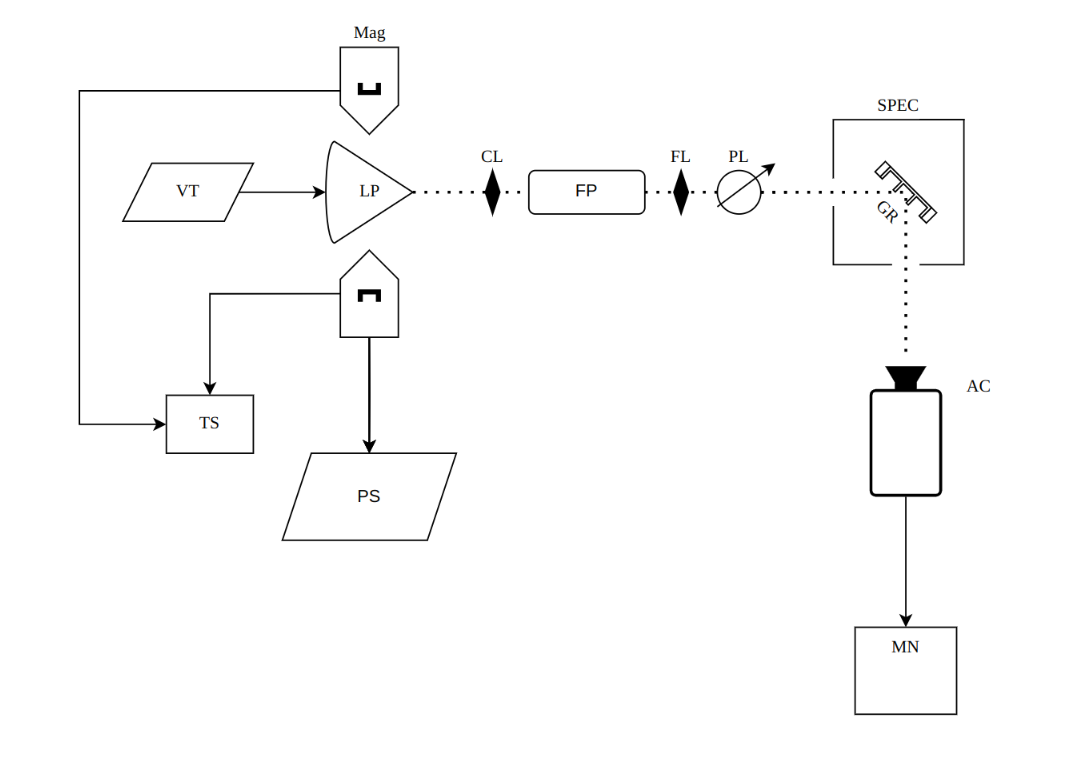
\includegraphics[width=0.9\linewidth]{1-zeeman_splitting/overleaf/images/Screenshot_20240913_094536.png}
    \caption{ \scriptsize{Neon discharge lamp (LP) with variable transformer (VT), high field magnet (Mag) with power supply (PS), a Tesla Meter (TS), a collimating lens (CL), the FABRY - PEROT interferometer (FP), a focusing lens (FL), a polarizer (Pl), a spectrograph (SPEC) with reflection grating (GR), and a analog camera (AC) connected to a monitor (MN) .} }
    \label{fig:enter-label}
\end{figure}

\end{center}

\begin{multicols}{2}

\section*{Theory \& Procedure }
{
The Zeeman effect is a phenomenon where when subjected to a magnetic field (\textbf{\textit{B}}), the total angular momentum (\textbf{\textit{J}}) splits into $2\textbf{\textit{J}} + 1$ components. The total angular momentum of an electron is a combination of its orbital angular momentum, due to its orbit around the nucleus, and its intrinsic spin. Each component of the total angular momentum generates a distinct magnetic moment, and their combined interaction produces a spin-orbit magnetic effect. This interaction results in energy level shifts that are proportional to the strength of the external magnetic field. To observe these shifts, we direct the light onto a Fabry-Perot interferometer (FP), which causes the incoming light to interfere constructively, producing multiple ring patterns, each with a different radius. This is done simultaneously for all wavelengths produced by the neon lamp. 
\\
\\
To begin the experiment, we first powered on the variable transformer (VT), which serves as the power supply for the neon lamp. Next, we activated the power supply (PS) responsible for generating the magnetic field in the magnets (Mag), as shown in Figure 1. The strength of this magnetic field was measured using a Tesla meter and a Hall Probe. We then calibrated the PS, ensuring that the current did not exceed 6 Amps. 
\\
\\
To accurately locate a specific wavelength, we used a 640 nm filter to establish a reference point, allowing us to determine the positions of other wavelengths relative to this reference. With this alignment complete, we were then prepared to begin collecting data.
\\
\\ 
When collecting data, we initially started with no external magnetic field and kept the independent axis $n$ at zero. We gradually increased the magnetic field until we observed double density in the spectral lines. At this point, we incremented the independent axis by 0.25 and recorded the corresponding magnetic field strength. We then continued to increase the magnetic field until single density was observed, after which we again incremented the independent axis by 0.25 and measured the magnetic field strength. This process was repeated until we reached the calibrated maximum set on the power supply (PS).
}


\section*{Analysis \& Results}
{
To calculate an average $g$ we found a best fit for the linear relationship between $n$ and the magnetic field strength \textbf{\textit{B}}. By taking the slope $m$ of the linear fitting and plugging it into \eqref{eq:first} we then found a g-factor for a set of measurements.
\begin{equation}\label{eq:first}
    g=\dfrac{h \nu_{\mathrm{f}}}{m \mu_{B}},
\end{equation}
where $h$ is Planck's constant, $\nu_{\mathrm{f}}$ is the free spectral range of the FP, and $\mu_{B}$ is the Bohr magneton. 
After repeating the measurement process 3 times we found the average g-factor $\overline{g}$ for each wavelength $\lambda$ and calculated a standard deviation $\sigma_{g}$ as well.


\begin{center}
\begin{tabular}{l|r|r|r}
$\lambda$ (\AA) & $\overline{g}$ & $\sigma_{g}$ & $\sigma$ within the accepted value \\ \hline
5852 & 1.113 & 0.009  \\
6074 & 1.558 & 0.013 \\
6164 & 1.488 & 0.010 & 14.8 \\
6266 & 1.094 & 0.007 & 13.5 \\
6533 & 0.879 & 0.004 & 52.5
\end{tabular}
\captionof{table}{$\overline{g}$, and $\sigma_{g}$ value for all $\lambda$ apparent enough to be measured. }
\end{center}

In our experiment, for the wavelengths that do have a documented accepted g-factor, our experimental value was consistently biased. We suspect this is mainly due to a systematic error. One of the many ways this error could have been caused is due to the Hall probe potentially being slightly tilted, or the Tesla meter not being completely zeroed out. 
}
\end{multicols}


\section*{Summary}
{
In all this lab aimed to investigate the splitting of spectral lines under the influence of an external magnetic field. By analyzing the shifts in energy levels corresponding to changes in a magnetic field, we quantified a g-factor for the observed transitions. The experiment was conducted using various advanced tools that may have contributed to any systematic errors we may have faced. Specifically, when using the Tesla Meter, it could be the case that the meter is not completely zeroed out, causing the reading of the field strength to be $\sim0.01$ off. Another systematic error is how we decide what single density is and what double density is. What I mean by this is, we could have chosen a point in which we believed to be double/single density and it could have very well been a point that is a transition point between the two. This may cause our data points to not entirely be at a equal relative distance from each other.
}
\begin{figure}
    \centering
    \subfloat{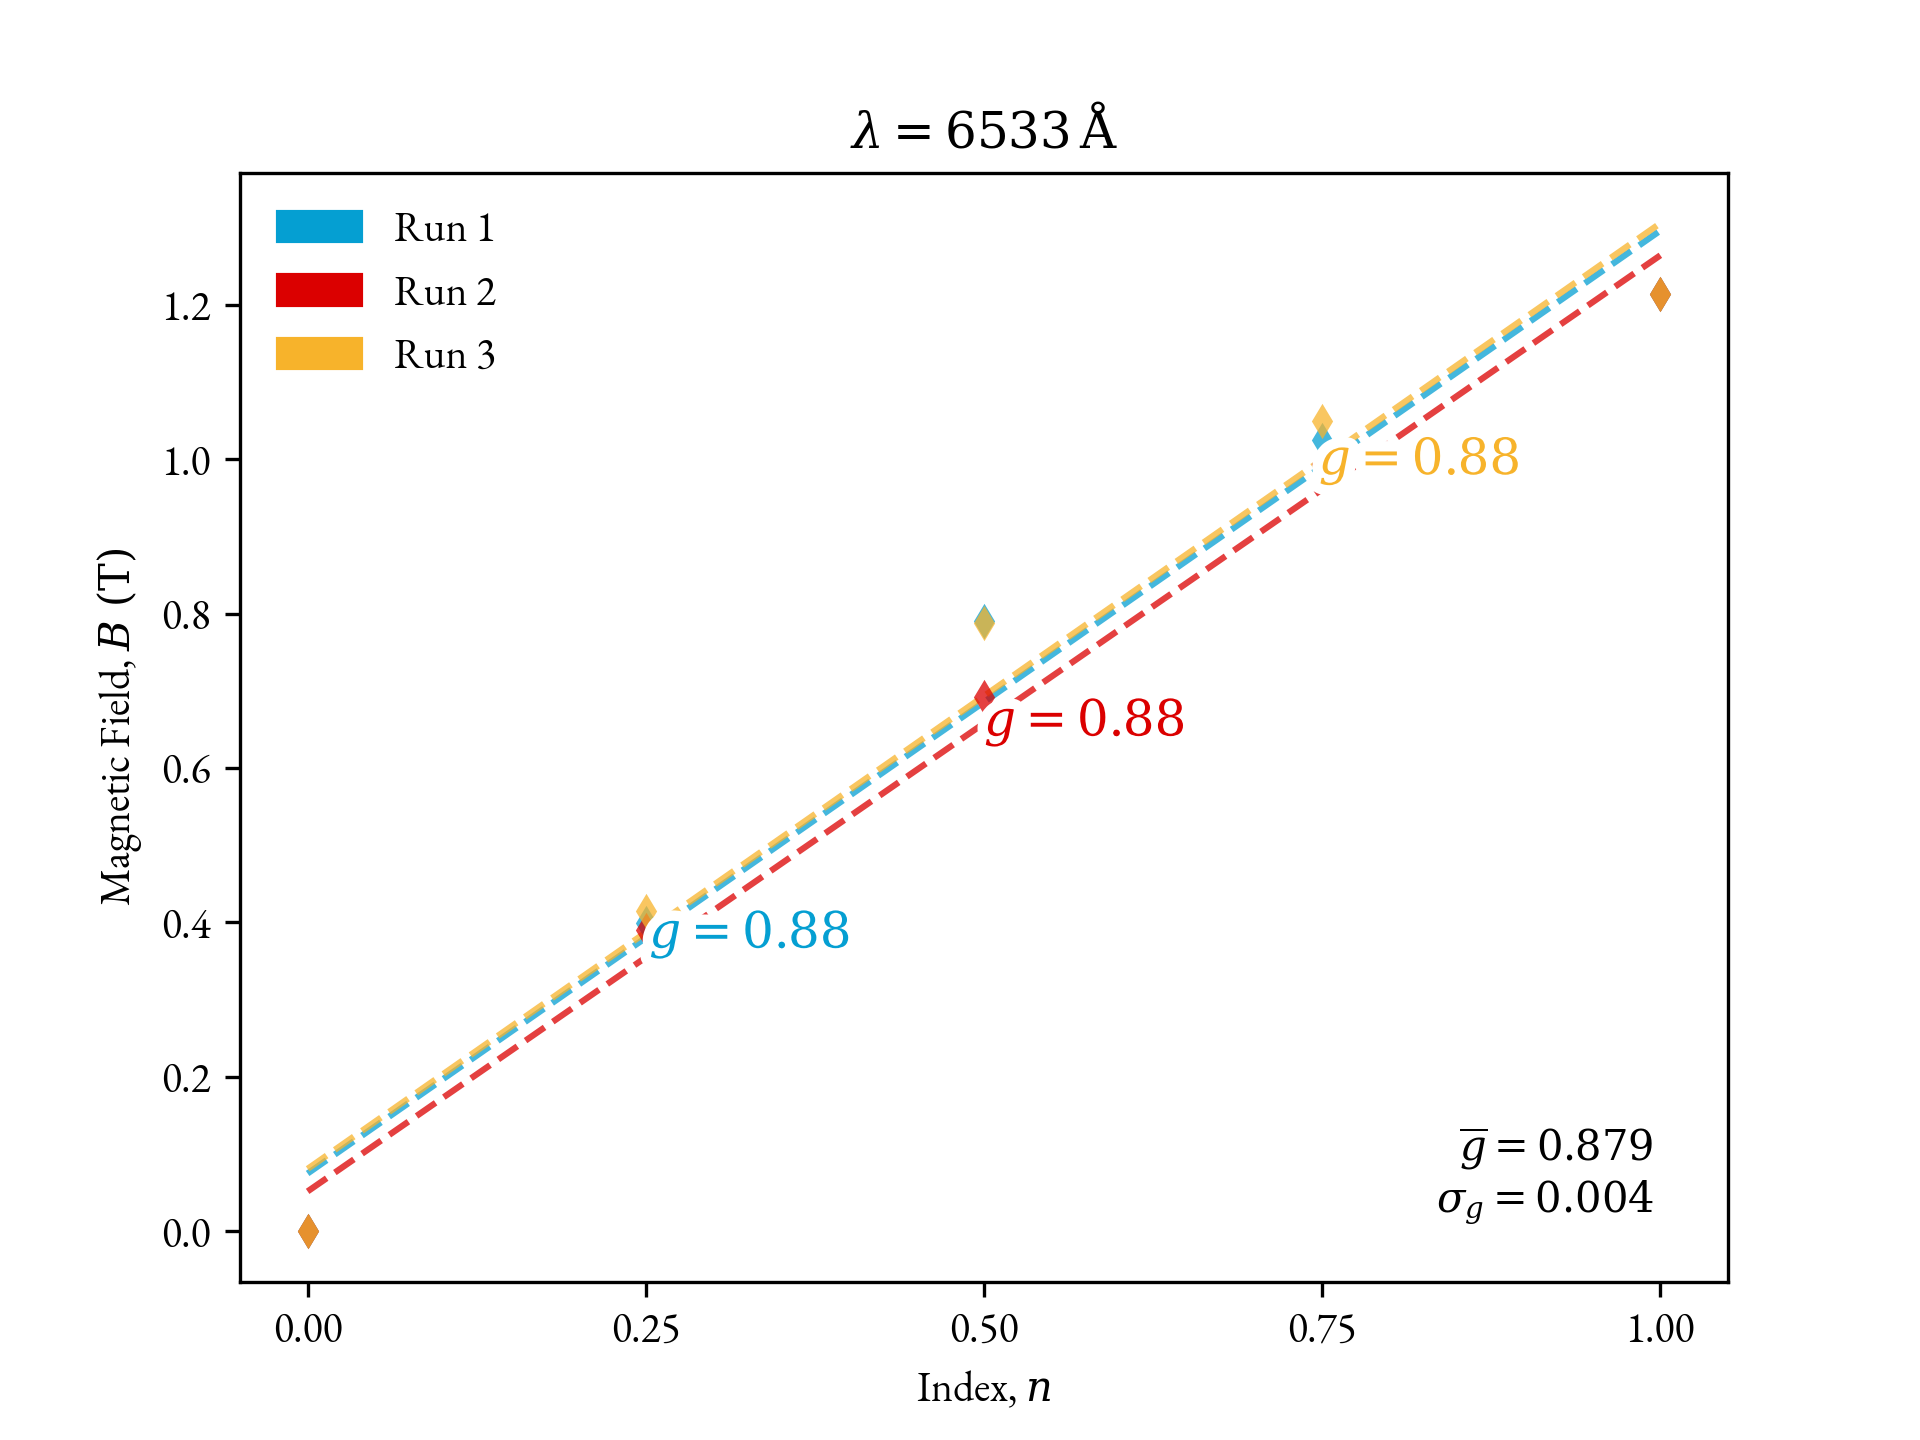
\includegraphics[width=90mm]{images/6533A.png}}
    \subfloat{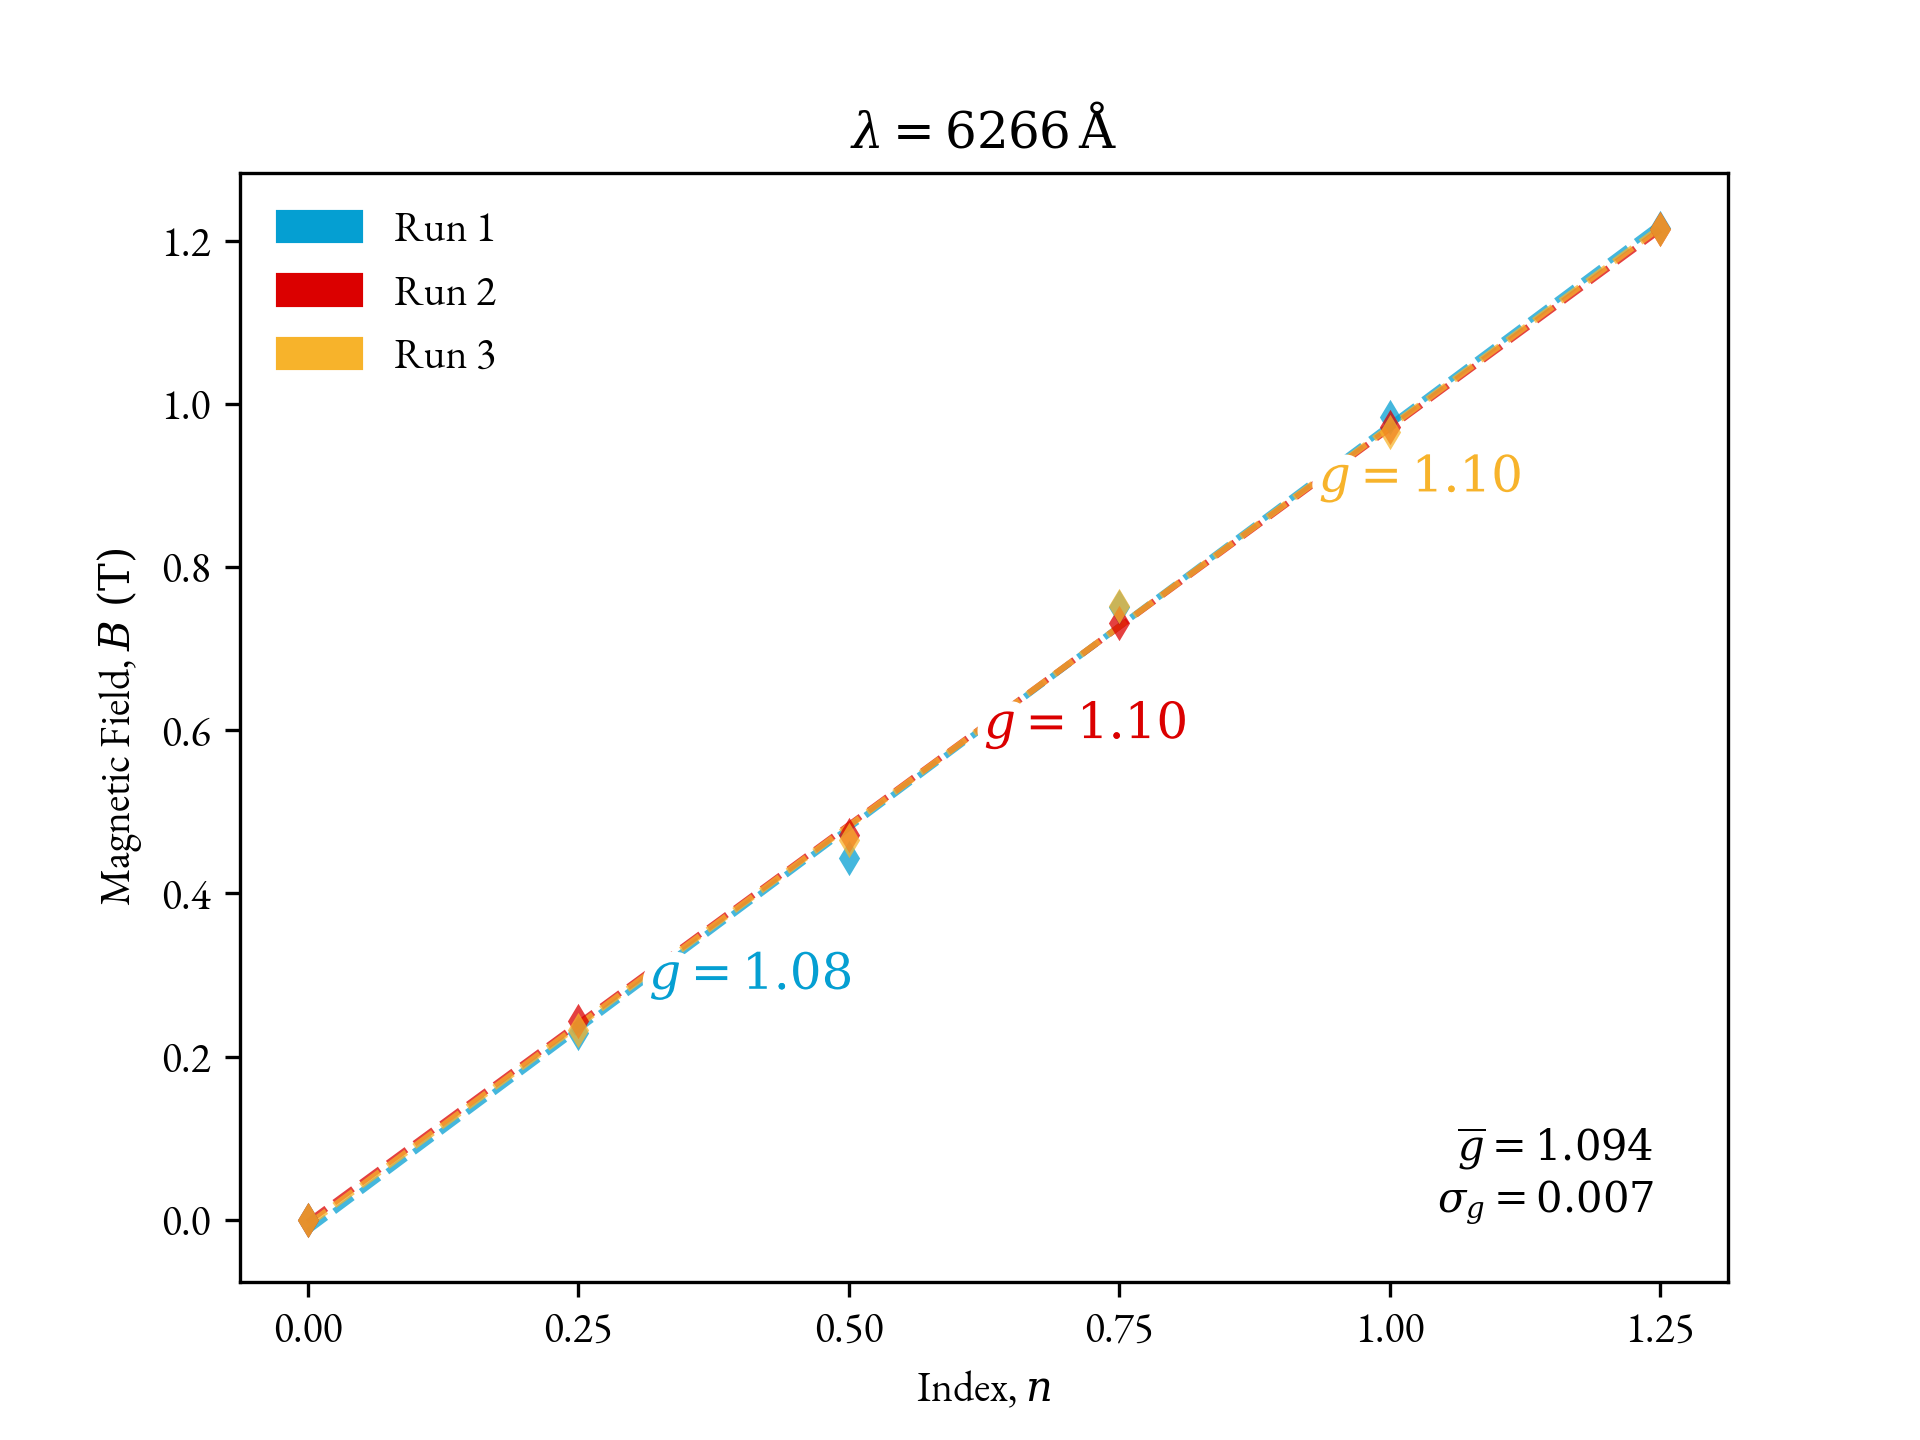
\includegraphics[width=90mm]{images/6266A.png}}
    \hspace{0mm}
    \subfloat{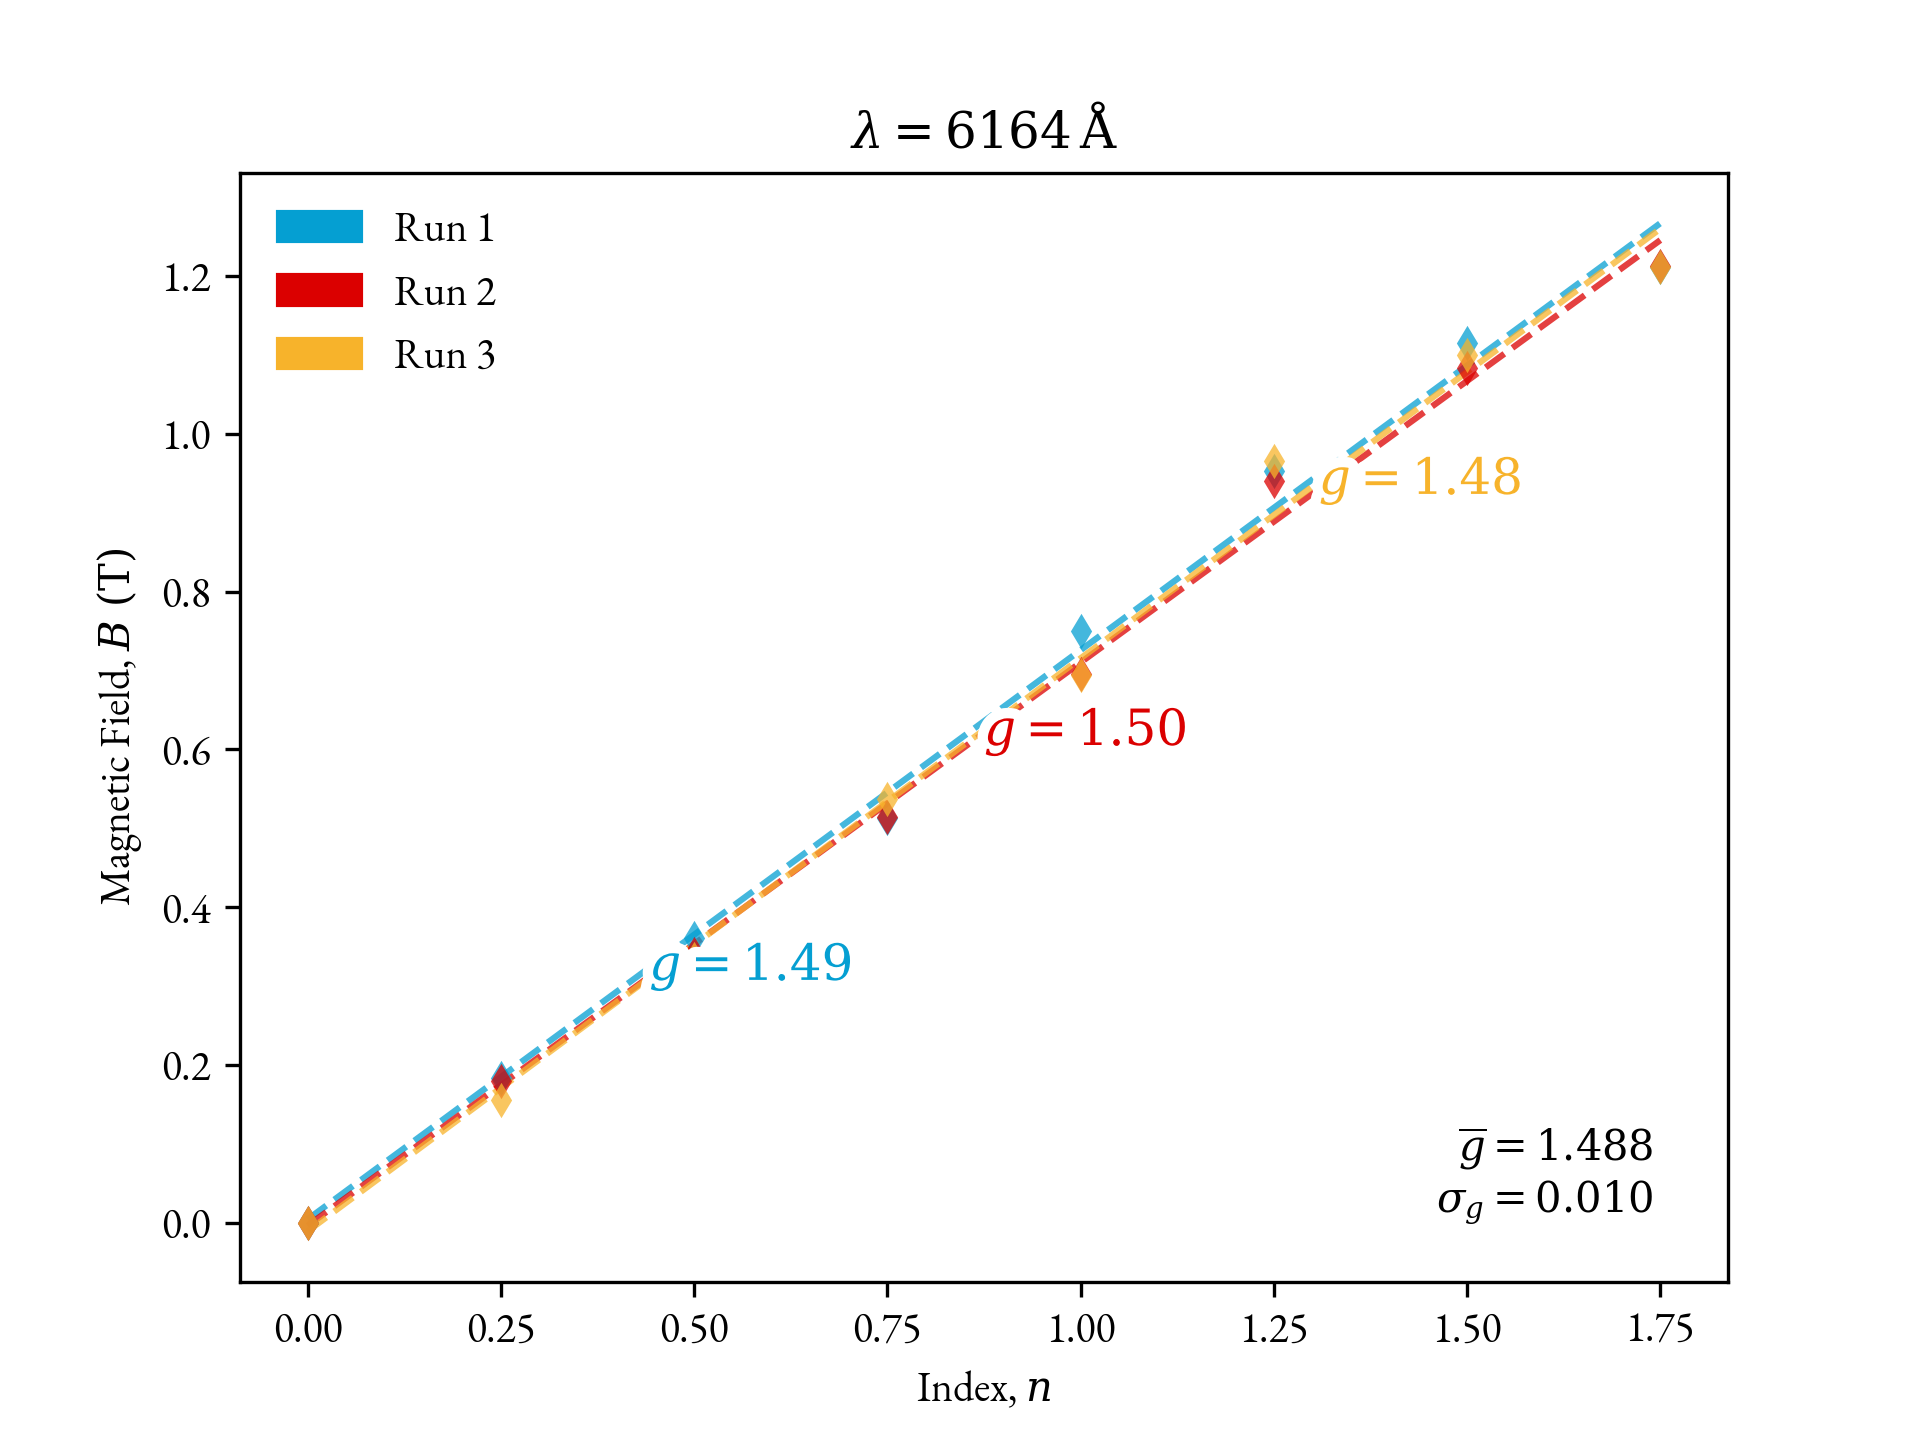
\includegraphics[width=90mm]{images/6164A.png}}
    \subfloat{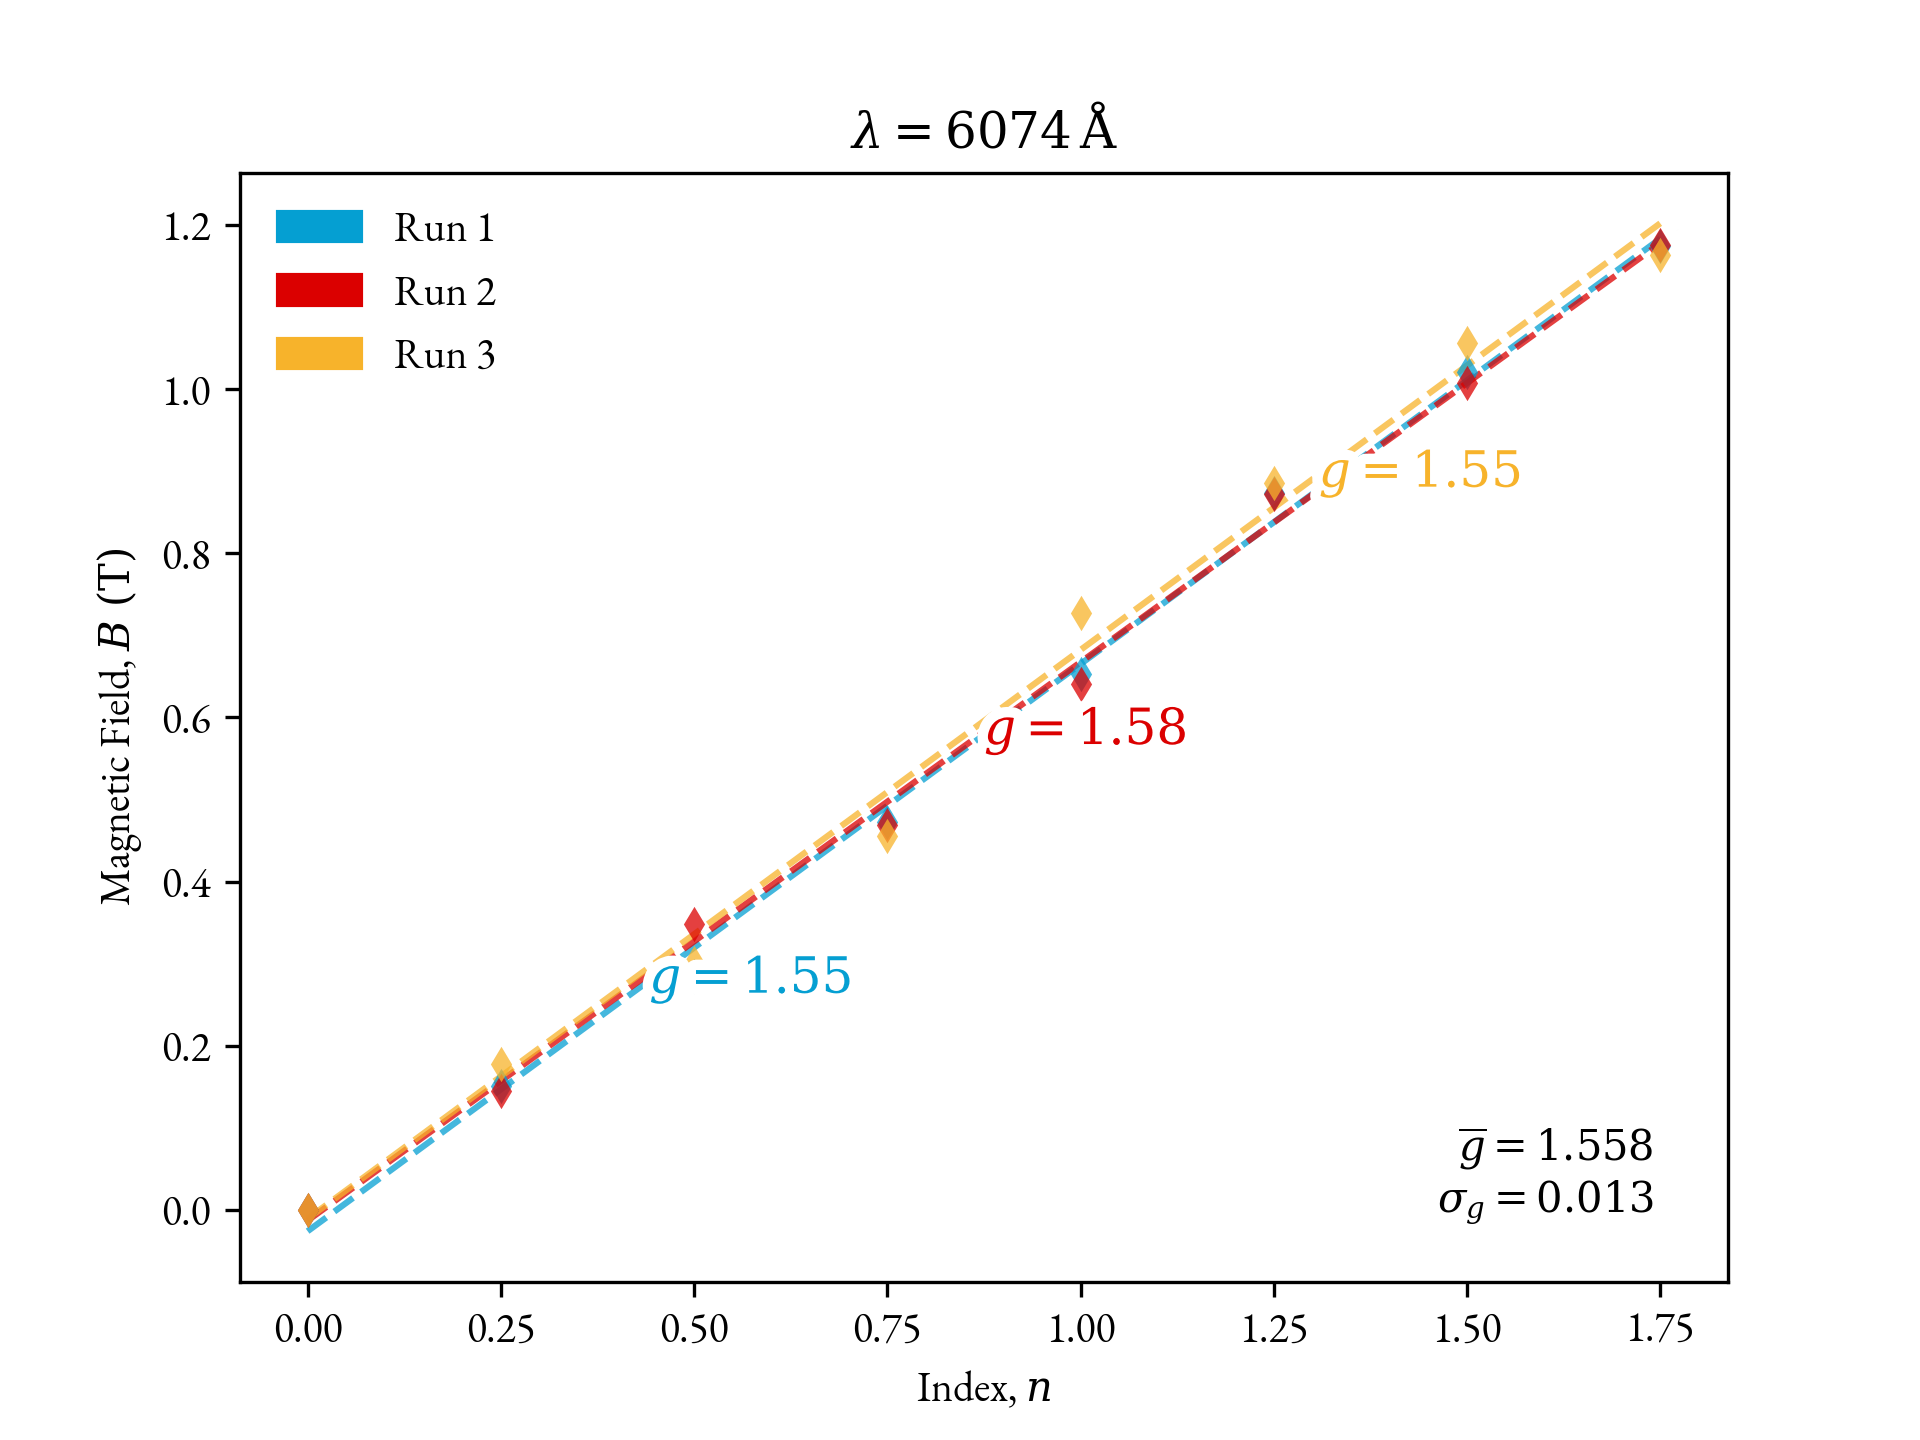
\includegraphics[width=90mm]{images/6074A.png}}
    \hspace{0mm}
    \subfloat{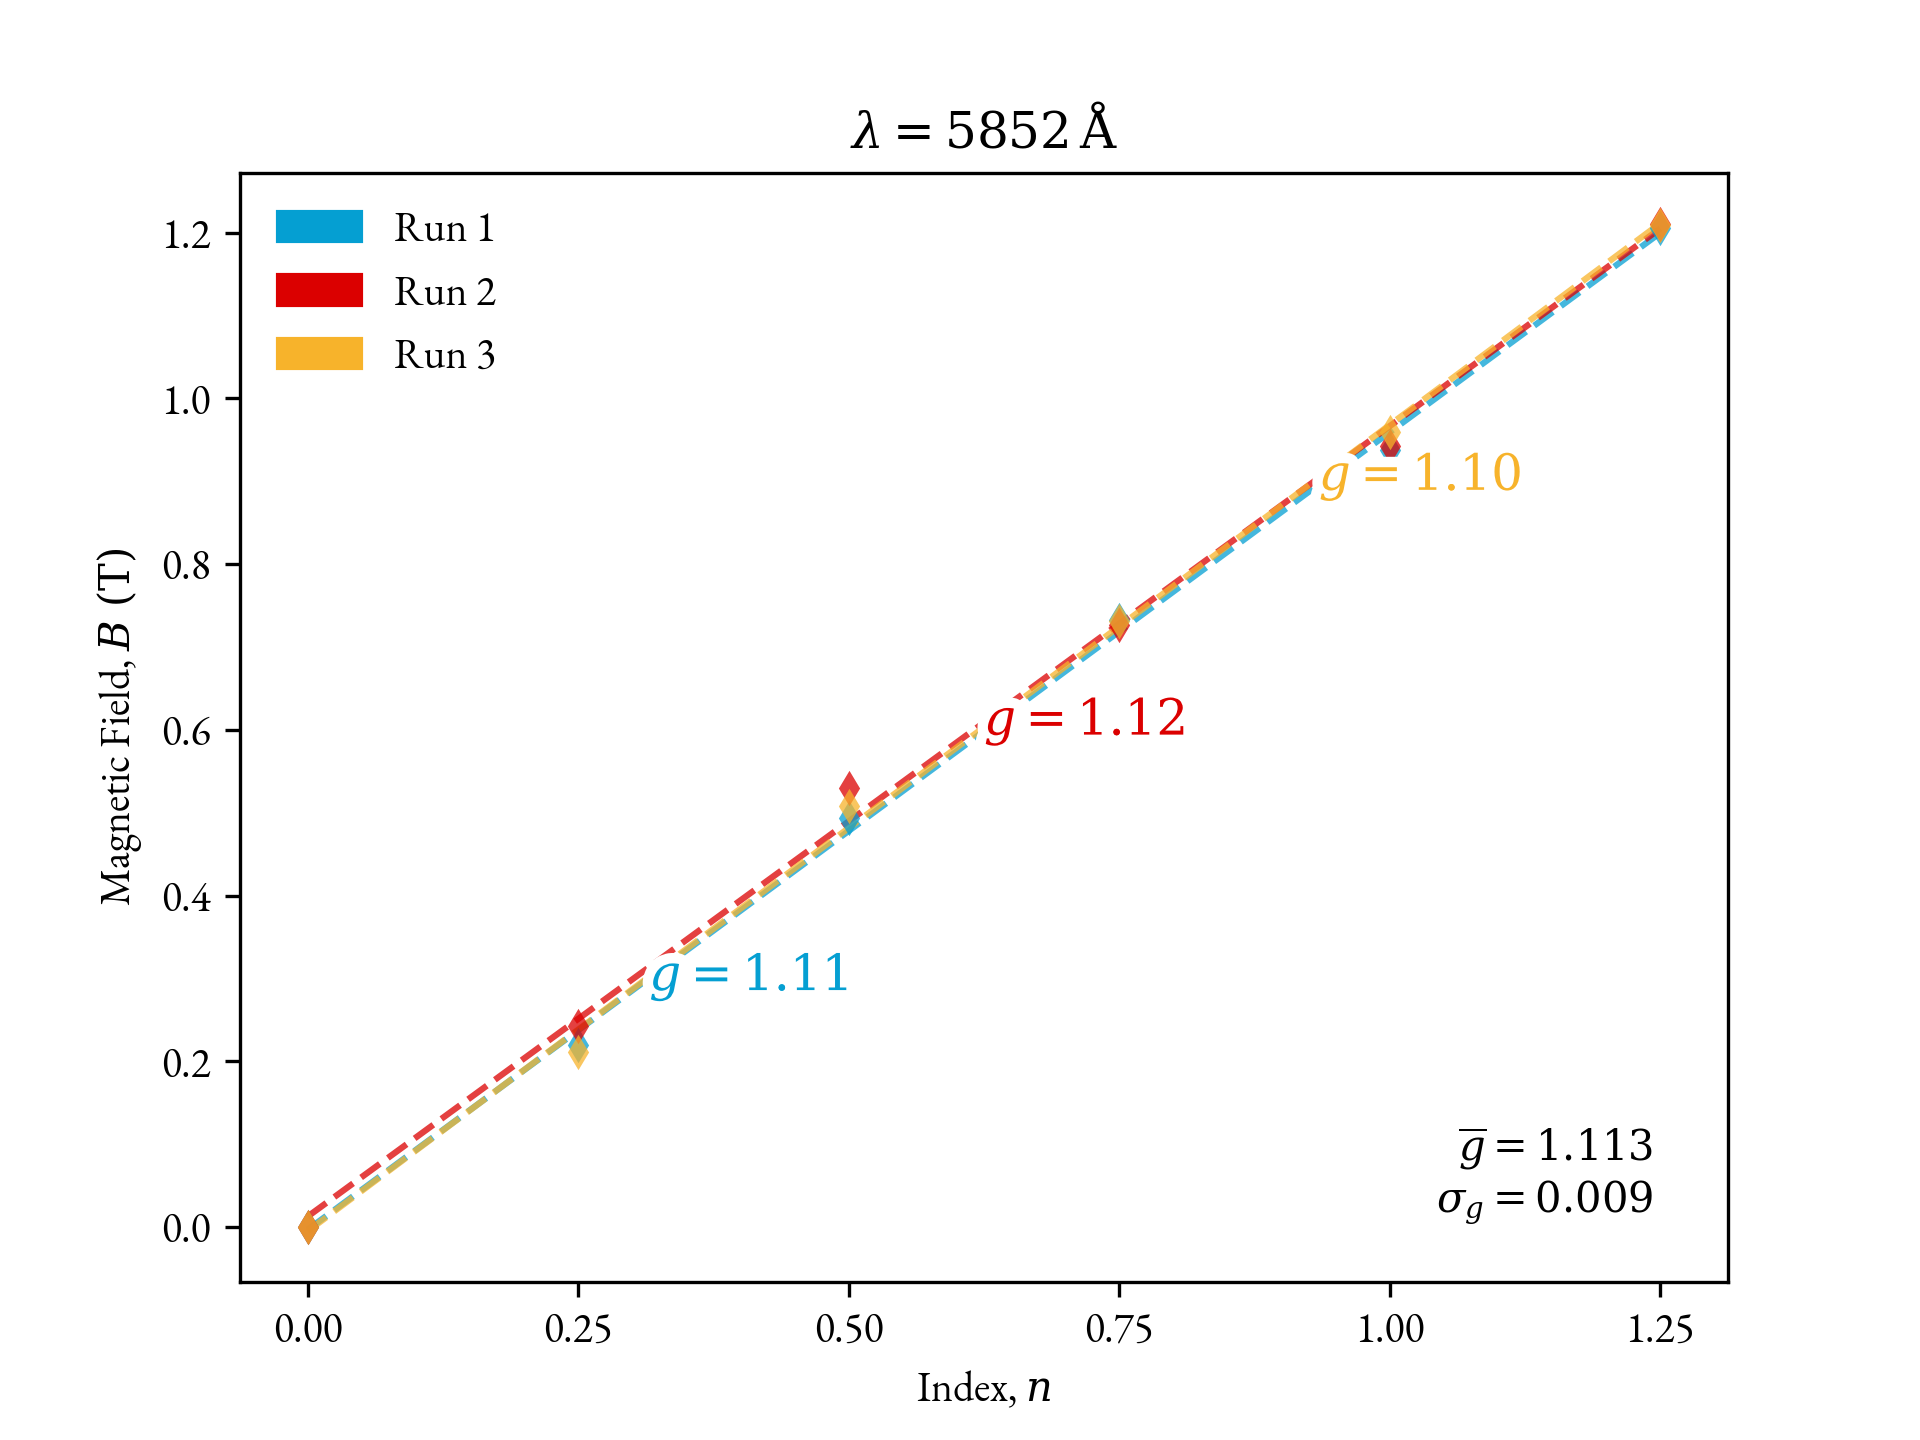
\includegraphics[width=90mm]{images/5852A.png}}
    \caption{ \scriptsize{ $g$, and $\sigma_{g}$ value for each run } }
    \label{fig:enter-label}
\end{figure}


\end{document}


